% !TEX program = xelatex
\documentclass[]{article}
\usepackage{float}
\usepackage{graphicx}
\usepackage[svgnames]{xcolor} 
\usepackage{fancyhdr}
\usepackage{fancyvrb}
\usepackage{forest}
\usepackage{tocloft}
\usepackage[hidelinks]{hyperref}
\usepackage{enumitem}
\usepackage[many]{tcolorbox}
\usepackage{listings }
\usepackage[a4paper, total={6in, 8in} , top = 2cm,bottom = 4cm]{geometry}
%\usepackage[a4paper, total={6in, 8in}]{geometry}
\usepackage{afterpage}
\usepackage{amssymb}
\usepackage{pdflscape}
\usepackage{textcomp}
\usepackage{xecolor}
\usepackage{rotating}
\usepackage[Kashida]{xepersian}
\usepackage[T1]{fontenc}
\usepackage{tikz}
\usepackage[utf8]{inputenc}
\usepackage{PTSerif} 
\usepackage{seqsplit}
\usepackage{changepage}

\usepackage{listings}
\usepackage{xcolor}
\usepackage{sectsty}

\setcounter{secnumdepth}{0}
 
\definecolor{codegreen}{rgb}{0,0.6,0}
\definecolor{codegray}{rgb}{0.5,0.5,0.5}
\definecolor{codepurple}{rgb}{0.58,0,0.82}
\definecolor{backcolour}{rgb}{0.95,0.95,0.92}
\definecolor{blanchedalmond}{rgb}{1.0, 0.92, 0.8}
\definecolor{brilliantlavender}{rgb}{0.96, 0.73, 1.0}
 
\NewDocumentCommand{\codeword}{v}{
\texttt{\textcolor{blue}{#1}}
}
\newcommand{\link}[2]{\href{#1}{\textcolor{blue}{#2}}}
\lstset{language=sql,keywordstyle={\bfseries \color{blue}}}

\lstdefinestyle{mystyle}{
    backgroundcolor=\color{backcolour},   
    commentstyle=\color{codegreen},
    keywordstyle=\color{magenta},
    numberstyle=\tiny\color{codegray},
    stringstyle=\color{codepurple},
    basicstyle=\ttfamily\normalsize,
    breakatwhitespace=false,         
    breaklines=true,                 
    captionpos=b,                    
    keepspaces=true,                 
    numbers=left,                    
    numbersep=5pt,                  
    showspaces=false,                
    showstringspaces=false,
    showtabs=false,                  
    tabsize=2
}

\lstset{style=mystyle}

 \settextfont[BoldFont={XB Zar bold.ttf}]{XB Zar.ttf}


\setlatintextfont[Scale=1.0,
 BoldFont={LiberationSerif-Bold.ttf}, 
 ItalicFont={LiberationSerif-Italic.ttf}]{LiberationSerif-Regular.ttf}





\newcommand{\inputsample}[1]{
    ~\\
    \textbf{ورودی نمونه}
    ~\\
    \begin{tcolorbox}[breakable,boxrule=0pt]
        \begin{latin}
            \large{
                #1
            }
        \end{latin}
    \end{tcolorbox}
}

\newcommand{\outputsample}[1]{
    ~\\
    \textbf{خروجی نمونه}

    \begin{tcolorbox}[breakable,boxrule=0pt]
        \begin{latin}
            \large{
                #1
            }
        \end{latin}
    \end{tcolorbox}
}

\newtcolorbox{mybox}[2][]{colback=red!5!white,
colframe=red!75!black,fonttitle=\bfseries,
colbacktitle=red!85!black,enhanced,
attach boxed title to top center={yshift=-2mm},
title=#2,#1}

\newenvironment{changemargin}[2]{%
\begin{list}{}{%
\setlength{\topsep}{0pt}%
\setlength{\leftmargin}{#1}%
\setlength{\rightmargin}{#2}%
\setlength{\listparindent}{\parindent}%
\setlength{\itemindent}{\parindent}%
\setlength{\parsep}{\parskip}%
}%
\item[]}{\end{list}}


\definecolor{foldercolor}{RGB}{124,166,198}
\definecolor{sectionColor}{HTML}{ff5e0e}
\definecolor{subsectionColor}{HTML}{008575}

\definecolor{listColor}{HTML}{00d3b9}

\definecolor{umlrelcolor}{HTML}{3c78d8}

\definecolor{subsubsectionColor}{HTML}{3c78d8}

\defpersianfont\authorFont[Scale=0.9]{XB Zar bold.ttf}

\defpersianfont\titr[Scale=1.5]{Lalezar-Regular.ttf}

\defpersianfont\fehrest[Scale=1.2]{Lalezar-Regular.ttf}

\defpersianfont\fehrestTitle[Scale=3.0]{Lalezar-Regular.ttf}

\defpersianfont\fehrestContent[Scale=1.2]{XB Zar bold.ttf}


\sectionfont{\color{sectionColor}}  % sets colour of sections
\subsectionfont{\color{subsectionColor}}  % sets colour of sections
\subsubsectionfont{\color{subsubsectionColor}}


\renewcommand{\labelitemii}{$\circ$}


\renewcommand{\baselinestretch}{1.1}


\renewcommand{\contentsname}{فهرست}

\renewcommand{\cfttoctitlefont}{\fehrestTitle}


\renewcommand\cftsecfont{\color{sectionColor}\fehrestContent\selectfont}
\renewcommand\cftsubsecfont{\color{subsectionColor}\fehrestContent\selectfont}
\renewcommand\cftsubsubsecfont{\color{subsubsectionColor}\fehrestContent\selectfont}
%\renewcommand{\cftsecpagefont}{\color{sectionColor}}

\setlength{\parskip}{1.2pt}

\begin{document}


%%% title pages
\begin{titlepage}
\begin{center}


\textbf{ \Huge{به نام خدا} }
        
\vspace{0.2cm}


\includegraphics[width=0.4\textwidth]{sharif1.png}\\
\vspace{0.2cm}
\textbf{ \Huge{\emph درس برنامه‌سازی پیشرفته} }\\
\vspace{0.25cm}
\textbf{ \Large{ توضیحات شبکه} }
\vspace{0.2cm}
       
 
      \large \textbf{دانشکده مهندسی کامپیوتر}\\\vspace{0.1cm}
    \large   دانشگاه صنعتی شریف\\\vspace{0.2cm}
       \large   ﻧﯿﻢ سال دوم 01-00 \\\vspace{0.10cm}
      \noindent\rule[1ex]{\linewidth}{1pt}
استاد:\\
    \textbf{{دکتر محمدامین فضلی}}



    \vspace{0.20cm}


    

\end{center}
\end{titlepage}
%%% title pages


%%% header of pages
\newpage
\pagestyle{fancy}
\fancyhf{}
\fancyfoot{}
\cfoot{\thepage}
\lhead{شبکه}
\rhead{
\includegraphics[width=0.1\textwidth]{sharif.png}\\
دانشکده مهندسی کامپیوتر
}
\chead{پروژه برنامه‌سازی پیشرفته}
%%% header of pages
\renewcommand{\headrulewidth}{2pt}

\KashidaOff



\tableofcontents

\newpage

 \Large \textbf{\\
}


\section*{{\titr مفاهیم شبکه}}
\addcontentsline{toc}{section}{{\fehrestContent مفاهیم شبکه}}
\subsection*{{\titr شبکه چیست؟}}
\addcontentsline{toc}{subsection}{{\fehrestContent شبکه چیست؟}}
شبکه به طور کلی به معنای ارتباط و اشتراک اطلاعات بین چند فرد یا چند شیء است. در زمینه فناوری اطلاعات هم به ارتباط بین چند سیستم کامپیوتری، نرم افزار یا سخت افزار با وسایل ارتباطی مثل کابل یا تجهیزات بیسیم، شبکه می گویند. در واقع شبکه مجموعه‌ای از سیستم‌ها است که از طریق یک کانال ارتباطی می‌توانند داده و منابع را به اشتراک بگذارند.
در ادامه، به معرفی مفاهیم مربوط به شبکه می‌پردازیم.

\subsection*{{\titr مفاهیم اولیه شبکه و ارتباط}}
\addcontentsline{toc}{subsection}{{\fehrestContent مفاهیم اولیه شبکه و ارتباط}}
\begin{itemize}
	\item \textbf{\lr{Node}:} در شبکه‌های کامپیوتری به هر کدام از سیستم‌ها \lr{Node} هم گفته می‌شود. \lr{Node}ها می‌توانند شامل کامپیوترهای شخصی، تلفن‌ها، پرینت سرورها و دیگر سخت‌ افزارهای مرتبط با شبکه باشند.
	\item \link{https://en.wikipedia.org/wiki/Network_packet}{\textbf{\lr{Packet}:}} به طور کلی در شبکه‌های کامپیوتری برای تبادل اطلاعات، داده‌های بزرگ به قسمت‌های کوچکتر تقسیم می‌شوند و هر یک از این قسمت‌ها را بسته یا packet‌ می‌نامند. هر packet که در شبکه ارسال می‌شود، دارای مشخصات و IP مربوط به مبدا و مقصد است. 
	\item \textbf{\lr{IP Address}:} هر میزبان در شبکه، یک آدرس مخصوص به خود به نام \lr{IP Address} دارد. این آدرس یکتاست و از ۴ عدد ۸ بیتی تشکیل شده است. وقتی سایتی را در مرورگر جست و جو می‌کنید، درخواستی همراه با IP‌ شما به آن سایت فرستاده می‌شود. سرور آن سایت نیز اطلاعات درخواستی را با کمک IP آدرس شما برایتان ارسال می‌کند.
	\item \link{https://www.cloudflare.com/learning/network-layer/what-is-a-computer-port/}{\textbf{\lr{Port}}:} فرض کنید کامپیوتر شما توسط برنامه‌های (process) مختلفی نیاز به برقراری ارتباط با شبکه دارد. در این صورت \lr{IP Address} به تنهایی پاسخگو نخواهد بود و از port استفاده می‌شود. پورت عددی است که برای شناسایی process خاصی که قصد دسترسی به شبکه را دارد استفاده می‌شود. در واقع به هر برنامه (process) که منتظر دریافت پیام از شبکه است (listening)، یک پورت نسبت داده می‌شود که با استفاده از آن، برنامه مقصد به صورت یکتا در کامپیوتر مشخص می‌شود.\\
	پورت و IP آدرس را می شود مانند شماره تلفن در نظر گرفت که IP آدرس کد شهر یا کشور است و پورت، باقی شماره تلفن در نظر گرفته می شود. کد شهر یا IP آدرس جهت شناسایی محدوده و منطقه تماس به کار می رود و قسمت باقی‌مانده یا پورت، شماره اختصاصی و یکتایی است که تماس با آن برقرار می‌شود.	
	\item \link{https://www.geeksforgeeks.org/socket-in-computer-network/}{\textbf{\lr{Socket}:}} به شکل ساده، سوکت ترکیبی از پورت و IP آدرس است. یک سوکت شامل هر دو گروه آدرس آی‌پی میزبان و پورت مربوط به یک برنامه است که با یک علامت جداکننده این دو مقدار از یکدیگر جدا شده اند (مثلا \lr{172.0.0.1:8000}). \\
	به تعبیر تخصصی تر، سوکت نقطه انتهایی یک ارتباط دوطرفه بین دو برنامه در حال اجرا در شبکه است. سوکت به یک عدد پورت متصل می شود تا لایه TCP شبکه بتواند برنامه مورد نظر برای ارسال اطلاعات را تشخیص دهد. در مثال شماره تلفن، سوکت مانند گوشی تلفن است. به این شکل که شماره مورد نظر و کد ناحیه را در گوشی وارد کرده و تماس را برقرار می‌کنید. زمانی که تماس پاسخ داده می‌شود، در واقع یک کانال ارتباطی بین شما و فردی که با او تماس گرفته‌اید، ایجاد می‌شود؛ به تعبیر ساده‌تر، کار سوکت ایجاد این کانال است. از طریق کانال ارتباطی ایجاد شده توسط سوکت، داده‌هایی در طول شبکه ارسال و دریافت میشوند. 
	\item \textbf{\lr{Protocol}:} کامپیوترها برای تبادل اطلاعات باید به توافق اولیه برسند که چطور اطلاعات ساختاربندی شود و هر طرف چطور و چه مقدار داده ارسال و دریافت می‌کند. تصور کنید کامپیوتری بسته ۸ بیتی می‌فرستد در حالی که کامپیوتر مقصد منتظر بسته ۱۶ بیتی است! پروتکل‌ها قوانین و استانداردهایی هستند که جهت جلوگیری از بروز چنین مشکلاتی در ایجاد ارتباط بین دو کامپیوتر در شبکه به کار می‌روند. 
\end{itemize}

\subsection*{{\titr لایه‌های شبکه}}
\addcontentsline{toc}{subsection}{{\fehrestContent لایه‌های شبکه}}
فرآیند ارتباط بین دو Node در شبکه را در نظر بگیرید. مهندسی این ارتباط بسیار پیچیده است. برای سهولت، کل فرآیند شبکه به وظایف کوچک تقسیم شده است. هر کار کوچک به یک لایه خاص اختصاص داده شده و هر لایه طوری کار می کند که تنها همان کار خاص را انجام دهد. هر لایه داده‌های ورودی را گرفته و داده‌های خروجی را به لایه بعدی ارسال می‌کند.

مدل \link{https://www.geeksforgeeks.org/layers-of-osi-model/}{OSI} يا \lr{Open System Interconnection} يك مدل مرجع براي ارتباط بين دو كامپيوتر است. طبق این مدل، ارتباط فرستادن و دریافت کردن پیام هر یک به هفت لایه تقسیم می‌شوند. 

زمانی که این لایه ها شروع به کار می‌کنند و از کامپیوتر مبدا می‌خواهند ارسال شوند لایه‌ها از بالا به پایین یعنی از لایه Application تشکیل شده و به لایه فیزیکی برای ارسال می‌رسند. اما در کامپیوتر مقصد دقیقا برعکس این موضوع است. از لایه فیزیکی به مقصد رسیده و در نهایت به لایه Application ختم می‌شود. 

\begin{figure}[H]
    \centerline{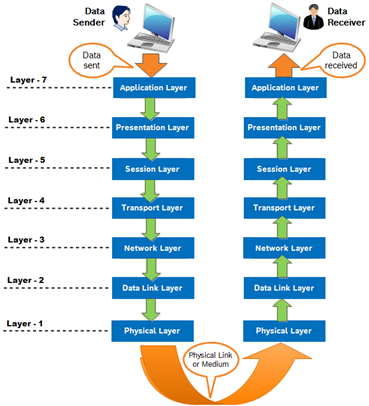
\includegraphics[scale=0.8]{resources/Layers.png}}
\end{figure}

در ادامه به طور مختصر کارکرد لایه‌ها توضیح داده شده است:

\begin{enumerate}
	\item \textbf{\lr{Application Layer}:} این لایه رابط بین کاربر و سیستم عامل محسوب می شود و همانطور که از اسمش پیداست، شما به وسیله این لایه با نرم‌افزارهای کاربردی ارتباط برقرار می‌کنید. در این جا داده‌هایی که باید در شبکه منتقل شوند تولید می‌شوند. پروتکل‌های لایه اپلیکیشن شامل دستوراتی برای اپلیکیشن‌های خاص هستند مثل HTTP و IMAP و FTP. مرورگرهای وب از https برای دانلود امن محتوا از وب سرور استفاده می‌کنند.
	\item \textbf{\lr{Presentation Layer (Translation Layer)}:} این لایه مانند مترجم داده‌های لایه application‌ را به فرمتی که برای انتقال در شبکه مورد نیاز است تبدیل می‌کند. به عنوان مثال تعیین می‌شود که اطلاعات چگونه رمزنگاری شوند، فشرده‌سازی شوند و قالب‌بندی شوند. 
	\item \textbf{\lr{Session Layer}:} این لایه مسئول پایه گذاری ارتباط (connection)، نگهداری از نشست‌ها (\link{https://www.computerhope.com/jargon/s/session.htm}{\lr{session}})، احراز هویت (\link{https://www.geeksforgeeks.org/authentication-in-computer-network/}{\lr{authentication}}) و مسائل امنیتی است.
	\item \textbf{\lr{Transport Layer}:} همان طور که می‌دانیم، در کامپیوتر ما چندین برنامه در حال ارتباط با شبکه هستند. پس اگر برنامه اول (از کامپیوتر اول) پیامی را به سمت کامپیوتر دوم می‌فرستد، این کامپیوتر باید به نحوی بفهمد که این پیام برای کدام برنامه است. این عملیات در لایه‌ی انتقال یا Transport پیاده سازی شده است. پروتکل‌های لایه انتقال، مشخص می‌کنند بسته‌ها چگونه ارسال و دریافت و تایید می‌شوند مانند TCP و UDP.
	\item \textbf{\lr{Network Layer}:} لایه‌ Network‌ مسیر انتقال داده از یک میزبان (\link{https://www.techtarget.com/searchnetworking/definition/host}{\lr{host}}) به دیگری را پیدا می‌کند. در واقع لایه‌ی network مسئول مسیریابی بسته‌ها یا \link{https://en.wikipedia.org/wiki/Routing}{\lr{packet routing}} بر اساس آدرس مبدا و مقصد هر packet است. از پروتکل‌های مربوط به این لایه می‌توان به  IPv4 و IPv6 اشاره کرد.
	\item \textbf{\lr{Data Link Layer}:} وظیفه این لایه آدرس دهی فیزیکی و ایجاد ارتباط مطمئن و بدون مشکل بین نود ها است. این لایه مکانیزم های مختلف برای مقابله با collision ها و error ها دارد.
	\item \textbf{\lr{Physical Layer}:} این لایه مرتبط با سخت افزار، کابل کشی سیمی، توان خروجی، تعداد پالس‌ها و غیره است و وظیفه انتقال سیگنال را بر عهده داشته و به محتویات هیچ کاری ندارد. سخت افزار موجود در این لایه از جنس انواع کابل ها، کارت شبکه و هاب است.
\end{enumerate}

\subsection*{{\titr معماری‌های شبکه}}
\addcontentsline{toc}{subsection}{{\fehrestContent معماری‌های شبکه}}
معماری شبکه در واقع مجموعه‌ای از قوانین و متودهایی برای طراحی منطقی و فیزیکی نرم افزار، سخت افزار، پروتکل‌ها و انتقال داده در شبکه است. دو مورد از معروف‌ترین معماری‌ها عبارتند از:

\begin{itemize}
	\item \textbf{\lr{Server/Client}:} در این معماری یک سرور مسئول پاسخ‌گویی به درخواست‌های(requests) کاربران یا کلاینت‌ها می‌باشد و با دریافت درخواست‌ها، پاسخ‌های(response) مناسب را به کاربران برمی‌گرداند. همچنین سرورها برنامه‌های خاصی را اجرا کرده و منابع خود را با کاربران به اشتراک می‌گذارند.	 سرور به منابع و اطلاعات اصلی برنامه دسترسی دارد و پردازش‌های اصلی داده ها در آن انجام شده و در نهایت نتیجه به شکل مناسبی به کلاینت اطلاع داده می‌شود.
	\begin{figure}[H]
		\centerline{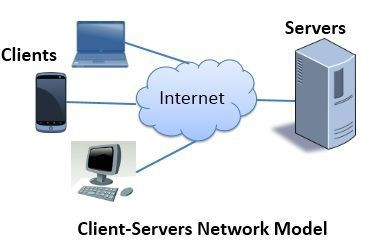
\includegraphics[scale=0.8]{resources/ClientServer.jpg}}
	\end{figure}
	\item \textbf{\lr{Peer-to-Peer (P2P)}:} نقطه مقابل معماری \lr{Client-Server} را می‌توان معماری \lr{Peer To Peer} یا نظیر به نظیر دانست. در معماری \lr{P2P}، دو یا چند کامپیوتر منابع خود را در قالب یک سیستم غیرمتمرکز به اشتراک می‌گذارند. در این سیستم دیگر ساختار سلسله مراتبی وجود ندارد. تمامی \lr{Node}های موجود، منابع خود را در اختیار دیگر \lr{Node}ها قرار می‌دهند. به همین دلیل هیچ \lr{Node}ای به Node دیگر ارجحیت ندارد. به هر Node در این شبکه، Peer می‌گویند. در واقع هر Node می‌تواند هم در نقش سرور (تامین کننده) و هم در نقش کلاینت (مصرف کننده) ظاهر شود.\\
	یکی از مزیت‌های اصلی شبکه‌های \lr{P2P} به نسبت شبکه‌های Client-Server، این است که در ساختار Client-Server اگر سرور دچار مشکل شود، کل خدمت‌رسانی دچار مشکل می‌شود. ولی در شبکه‌های \lr{P2P} اگر یک سیستم خراب شود، براحتی سیستم دیگری را می‌توان جایگزین آن کرد.\\
	هم‌چنین برای گسترش شبکه Client-Server، باید هزینه زیادی را صرف ارتقا سرور کنیم. ولی این کار در شبکه \lr{P2P} به دلیل غیرمتمرکز بودن آن، به راحتی قابل انجام است.\\
	از طرف دیگر در سیستم client-server یک سرور فایل اختصاصی سطوح دسترسی متفاوتی را برای کلاینت‌ها فراهم می‌کند که به نسبت سیستم‌های peer to peer که امنیت توسط کاربر نهایی اداره می‌شود از امنیت بیشتری برخوردار است. همچنین شبکه‌های \lr{peer to peer} با افزایش تعداد نودها دچار اختلال در سطح عملکرد می‌شوند، اما سیستم‌های client-server باثبات تر هستند.
	\begin{figure}[H]
		\centerline{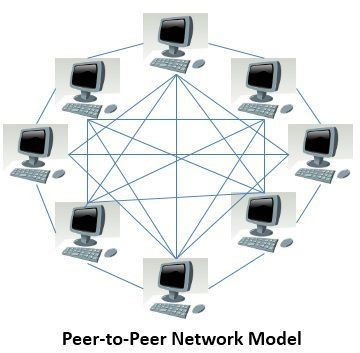
\includegraphics[scale=0.8]{resources/p2p.jpg}}
	\end{figure}
\end{itemize}

\subsection*{{\titr توپولوژی‌های شبکه}}
\addcontentsline{toc}{subsection}{{\fehrestContent توپولوژی‌های شبکه}}
توپولوژی‌های شبکه ارتباط اجزای موجود در شبکه و ارتباط آن‌ها را با همدیگر نشان می‌دهد. در این بخش به بررسی برخی توپولوژی‌های موجود می‌پردازیم:

\begin{itemize}
	\item \link{https://en.wikipedia.org/wiki/Bus_network}{\textbf{\lr{Bus Topology}:}} در این توپولوژی، هر Node به یک کابل متصل می‌باشد و داده‌ها در یک جهت منتقل می‌شوند و به Node های دیگر می‌رسند.
	از مزایای این روش می‌توان به مقرون به‌صرفه و ساده بودن پیاده سازی آن اشاره کرد. در مقابل، از کار افتادن کل سیستم در صورت قطع شدن کابل اصلی و کندتر بودن شبکه به نسبت توپولوژی‌های دیگر اشاره کرد.
	\begin{figure}[H]
		\centerline{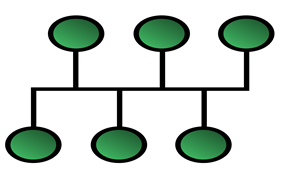
\includegraphics[scale=0.8]{resources/bus.png}}
	\end{figure}
	\item \link{https://en.wikipedia.org/wiki/Bus_network}{\textbf{\lr{Ring Topology}:}} در این توپولوژی، هر Node دقیقا به دو Node دیگر وصل می‌شود و ساختاری حلقه‌ای پدید می‌آورد. در این توپولوژی یک توکن در حال حرکت است و هر \lr{Node}ای که توکن را در اختیار داشته باشد قادر به ارسال پیام است. پیام‌ها در این توپولوژی در یک جهت در حال حرکت هستند و شبکه ابتدا و انتهایی ندارد و اطلاعات در یک حلقه منتقل می‌شوند. همچنین به دلیل اینکه اطلاعات از همه Nodeها در حال عبور هستند، از \lr{repeater}ها استفاده می‌شود که مانع از دست رفتن اطلاعات در این تبادلات طولانی باشد.\\
	از معایب این روش می‌توان به حساس بودن آن به کارکرد درست همه Node هاست. از آنجایی که داده‌ها از همه Nodeها عبور می‌کنند، ضروری است که همه \lr{Node}ها اطلاعات را به درستی دریافت و سپس ارسال کنند و در غیر اینصورت کل شبکه از کار می‌افتد. همچنین عیب‌یابی در این توپولوژی هم سخت‌تر از دیگر توپولوژی‌هاست.\\
	از طرفی راحتی نصب و نگه‌داری این شبکه و همچنین امنیت اطلاعات در شبکه‌هایی با حجم بالای داده به دلیل استفاده از توکن از مزایای این روش به حساب می‌آیند.
	\begin{figure}[H]
		\centerline{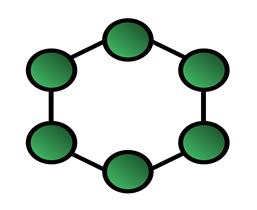
\includegraphics[scale=0.8]{resources/ring.png}}
	\end{figure}
	\item \link{https://en.wikipedia.org/wiki/Star_network}{\textbf{\lr{Star Topology}:}} در این توپولوژی نیز، تمام Nodeها به صورت جداگانه به یک Hub متصل می‌شوند. \lr{Hub}ها اجزایی در شبکه هستند که داده‌ها را به همه \lr{Node}های متصل به خودشان ارسال می‌کنند. همچنین خود Hub به‌عنوان repeater نیز عمل می‌کند.
	از مزایای این روش نیز می‌توان به عیب‌یابی ساده‌تر به دلیل متمرکز بودن سیستم، عملکرد سریع شبکه با \lr{Node‌}های کم و وابسته نبودن شبکه به عملکرد درست همه \lr{Node}ها می‌باشد. همچنین می‌توان به وابسته بودن شبکه به عملکرد درست Hub و هزینه‌بالای پیاده سازی آن به عنوان معایب آن اشاره کرد.
	\begin{figure}[H]
		\centerline{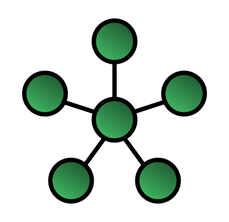
\includegraphics[scale=0.8]{resources/star.png}}
	\end{figure}
	\item \link{https://en.wikipedia.org/wiki/Mesh_networking}{\textbf{\lr{Mesh Topology}:}} در این توپولوژی، هر Node به مانند یک Router عمل می‌کند و با اتصالاتی که به دیگر \lr{Node}ها دارد اطلاعات را در شبکه منتقل می کند. توپولوژی Mesh بسته به اینکه \lr{Node}ها به چند Node دیگر وصل شده‌اند به ۲ نوع تقسیم می‌شوند:
	\begin{itemize}
		\item \lr{Partial}: در این توپولوژی، \lr{Node}ها به همه \lr{Node}های دیگر متصل نیستند.
		\item \lr{Full}: برخلاف \lr{partial}، هر \lr{Node} به همه \lr{Node}های دیگر وصل شده است.
	\end{itemize}
	همچنین بسته به منطق انتقال داده نیز می‌توان دو دسته‌بندی زیر را ارائه داد:
	\begin{itemize}
		\item \lr{Rountig}:  دستگاه ها بر اساس نیاز شبکه، یک منطق مسیریابی (routing) خواهند داشت. به عنوان مثال یکی از منطق های مسیریابی می تواند انتخاب بر اساس کوتاه ترین مسیر باشد
		\item \lr{Flooding}:  اطلاعات یکسان به تمامی دستگاه های شبکه منتقل می شود، بنابراین به هیچ مسیر یابی منطقی نیاز نیست
	\end{itemize}
	در این توپولوژی، امنیت داده‌ها و \lr{Node}ها بالاست و همچنینرعیب‌یابی سیستم نیز ساده است. درمقابل، به دلیل تعداد زیاد ارتباطات، هزینه و حجم کابل‌ها زیاد است.
	\begin{figure}[H]
		\centerline{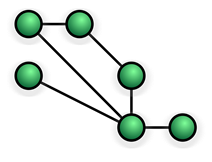
\includegraphics[scale=0.8]{resources/mesh.png}}
	\end{figure}
	\item \link{https://en.wikipedia.org/wiki/Tree_network}{\textbf{\lr{Tree Topology}:}} این توپولوژی یکی از بهترین انتخاب‌ها برای شبکه‌های بزرگ است. در این توپولوژی \lr{Node}ها به‌صورت سلسله مراتبی به یکدیگر وصل شده‌اند و در راس آن‌ها، یک دستگاه مرکزی وجود دارد. این شبکه حداقل باید ۳ سطح داشته باشد.\\
	مدیریت و نگه‌داری این شبکه بسیار ساده است و همچنین اضافه کردن Node جدید به شبکه نیز بدون دردسر است. در مقابل، این سیستم وابسته به دستگاه مرکزی است و همچنین حجم کابل استفاده شده نیز بالاست.
	\begin{figure}[H]
		\centerline{\includegraphics[scale=0.8]{resources/tree.png}}
	\end{figure}
\end{itemize}
\subsection*{{\titr اینترنت به عنوان یک شبکه و جابه‌جایی اطلاعات در اینترنت}}
\addcontentsline{toc}{subsection}{{\fehrestContent اینترنت به عنوان یک شبکه و جابه‌جایی اطلاعات در اینترنت}}

اطلاعات برای انتقال در بستر اینترنت، ابتدا به بسته‌های کوچکی به نام  Packet تقسیم می‌شوند. این بسته‌ها طی یک سفر طولانی به مقصد می‌رسند و دوباره با هم جمع شده و پیام اصلی را تشکیل می‌دهند.
ابتدا پکت‌ها با وارد شدن به router و modem هایی که به ارسال کننده پیام به آن متصل است، وارد شبکه \lr{ISP (Internet Service Provider)} می‌شود. شبکه‌ای که ISP ها باهمدیگر تشکیل می‌دهند، یک شبکه تقریبا بزرگ است که اکثر پیام‌ها در این شبکه قرار دارند. پکت‌ها با وارد شدن در این شبکه با توجه به دیتایی که در Header خود دارند، مسیریابی می‌شوند. الگوریتم‌های مسیریابی باید پکت‌ها را در کمترین زمان به مقصد برسانند. درنهایت، پکت‌ها از شبکه ISP ها خارج شده و با ورود به \lr{router}ها، به دستگاه مقصد که متصل به آن روتر است فرستاده می‌شود. در نهایت، یک Acknowledgment از گیرنده به فرستنده پیام ارسال می‌شود که نشان دهد پیام به درستی به گیرنده رسیده است.
شکل زیر یک شمای کلی از مسیری که پکت طی می‌کند را نشان می‌دهد. (\link{https://www.washingtonpost.com/graphics/national/security-of-the-internet/bgp/}{این لینک})

\begin{figure}[H]
	\centerline{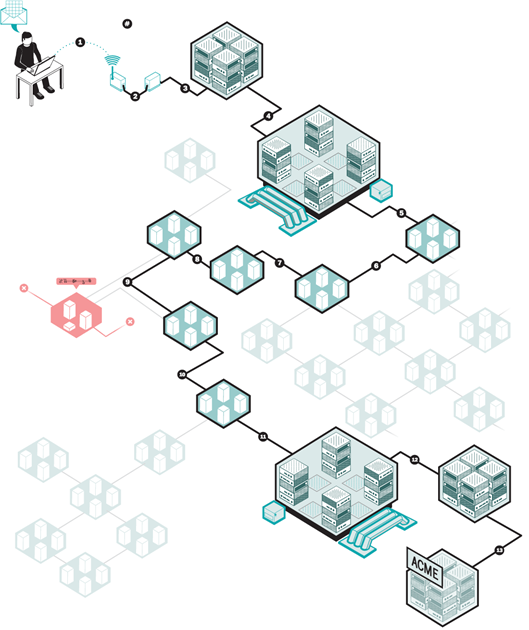
\includegraphics[scale=1]{resources/Dataflow.png}}
\end{figure}

\end{document}







